\section{Version 0.4}
The goal of this iteration and version was to implement the possibility to limit access to a users books. This was done by creating an assumption with questions to be answered, select the the user stories needed to support that feature and measure the use.

\subsection{Assumption and questions}
The assumption for this version was "Users only want to share books with a selection of other users"

In order to confirm this assumption, the team created a set of questions to be answered:

\begin{enumerate}

  \item Do users want to exclude users from borrowing their books?
  \item Do users want to to know the people they share books with?
  \item Do users need a crowd to share a book?
  \item Are users interested in organizing their network in a crowd form?
  \item Is security more important than efficiency?
  \item Do users want the ability share books with users that do not have the application?
  \item Do users want to share all their books with all users in their crowds, or be able to customize which books are available in a certain crowd?
  \item Are users more interested in which books are in a crowd, or the members?
\end{enumerate}


\subsection{Planning and design}

Based on the assumption, the team had to select a set of user stories needed to allow users to limit the access to their books. These user stories would be implemented in the mobile applications and the \gls{backend}. This would allow the team to measure the usage of the application in order to get and indication of whether the users wanted the crowd feature, or not.

A survey trying to answer the questions was created in order to get feedback from potential users. The feedback was used to discover what level of security and restrictions users wanted for their books. The survey was added to the website, linked on Facebook, and distributed to the \gls{IDI} at \gls{NTNU}.

Design sketches were made based on the features to be implemented, internal discussions, and feedback from Netlight employees. These sketches were used in \gls{guerrilla test} at the university. After having conducted usability tests with students in all previous versions, it was apparent that students had little trouble using the application, and the team realised that they were not necessarily representative users. Therefore it was decided to find test users who were less used to mobile platforms. The usability tests were performed with employees at \gls{IDI}, and the results were noticeably different. The users spent more time trying to figure out how to navigate the application, and one user did not manage to complete the tasks given. The design was revised, and new tests were conducted. The test users found the new design more intuitive.

\begin{figure}
    \centering
    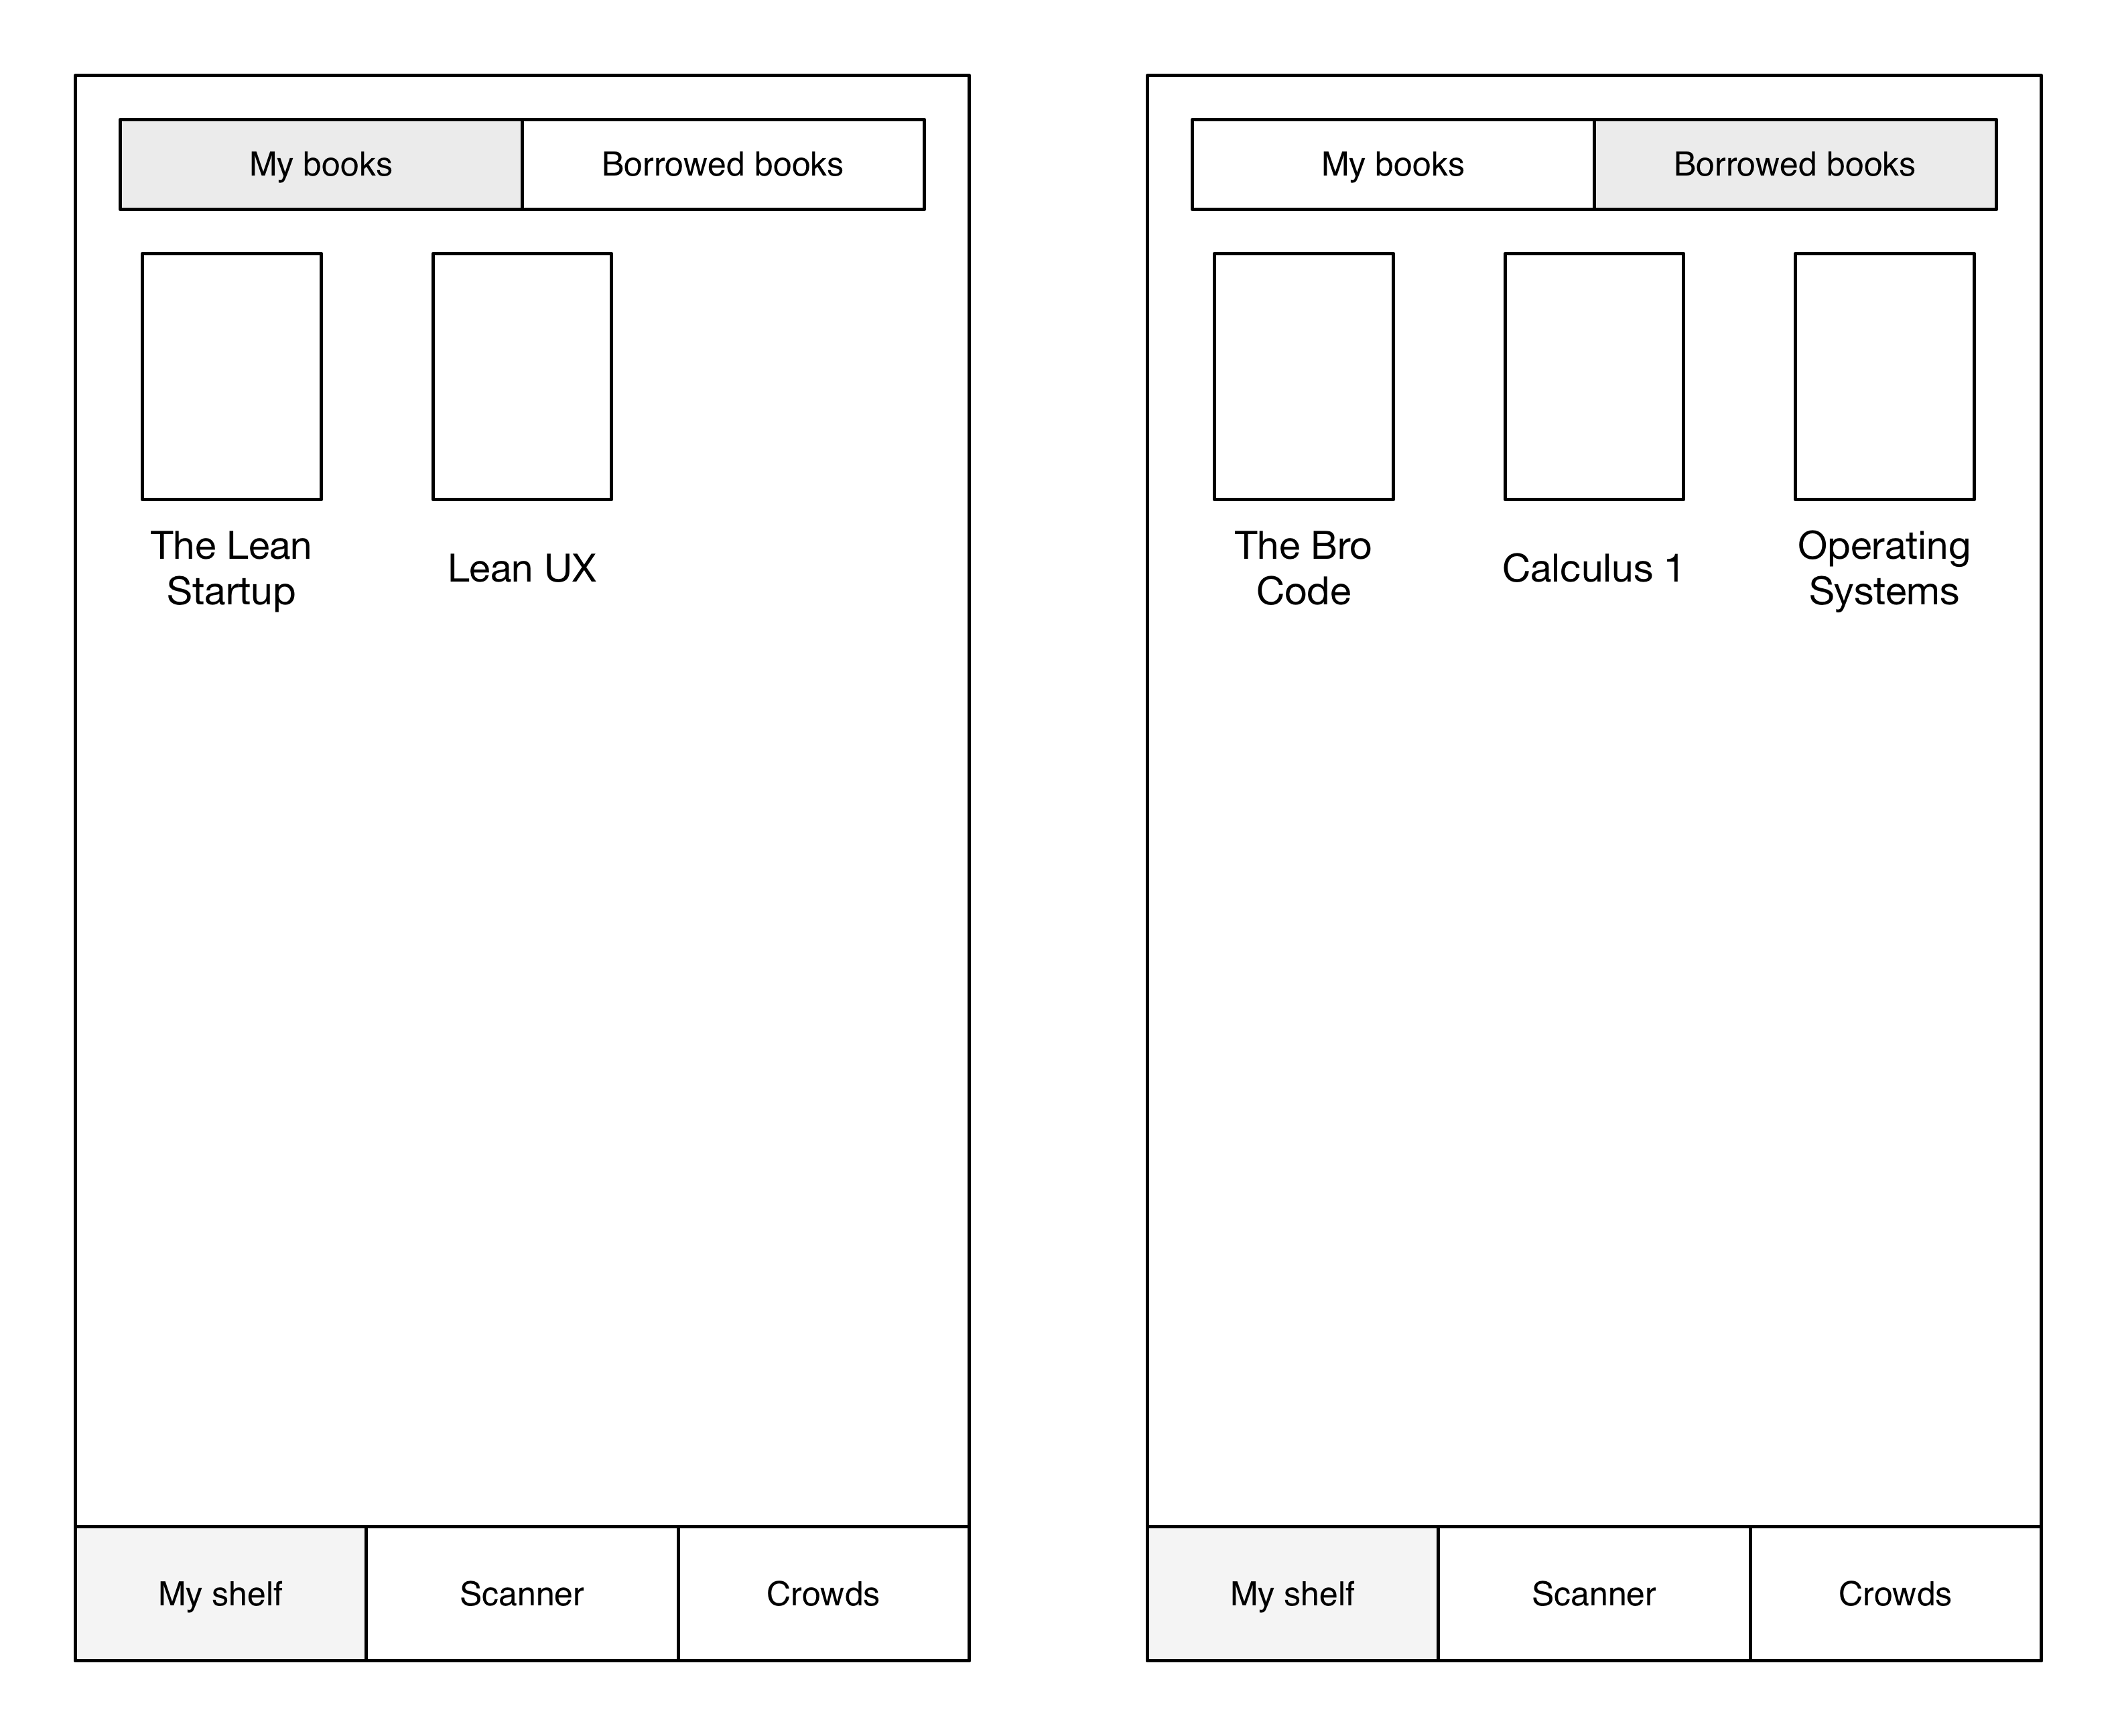
\includegraphics[height=5cm]{figs/v04/Shelf.png}
    \caption{The shelf view where the user can see all its books}
    \label{fig:ios-shelf}
\end{figure}

\begin{figure}
\centering
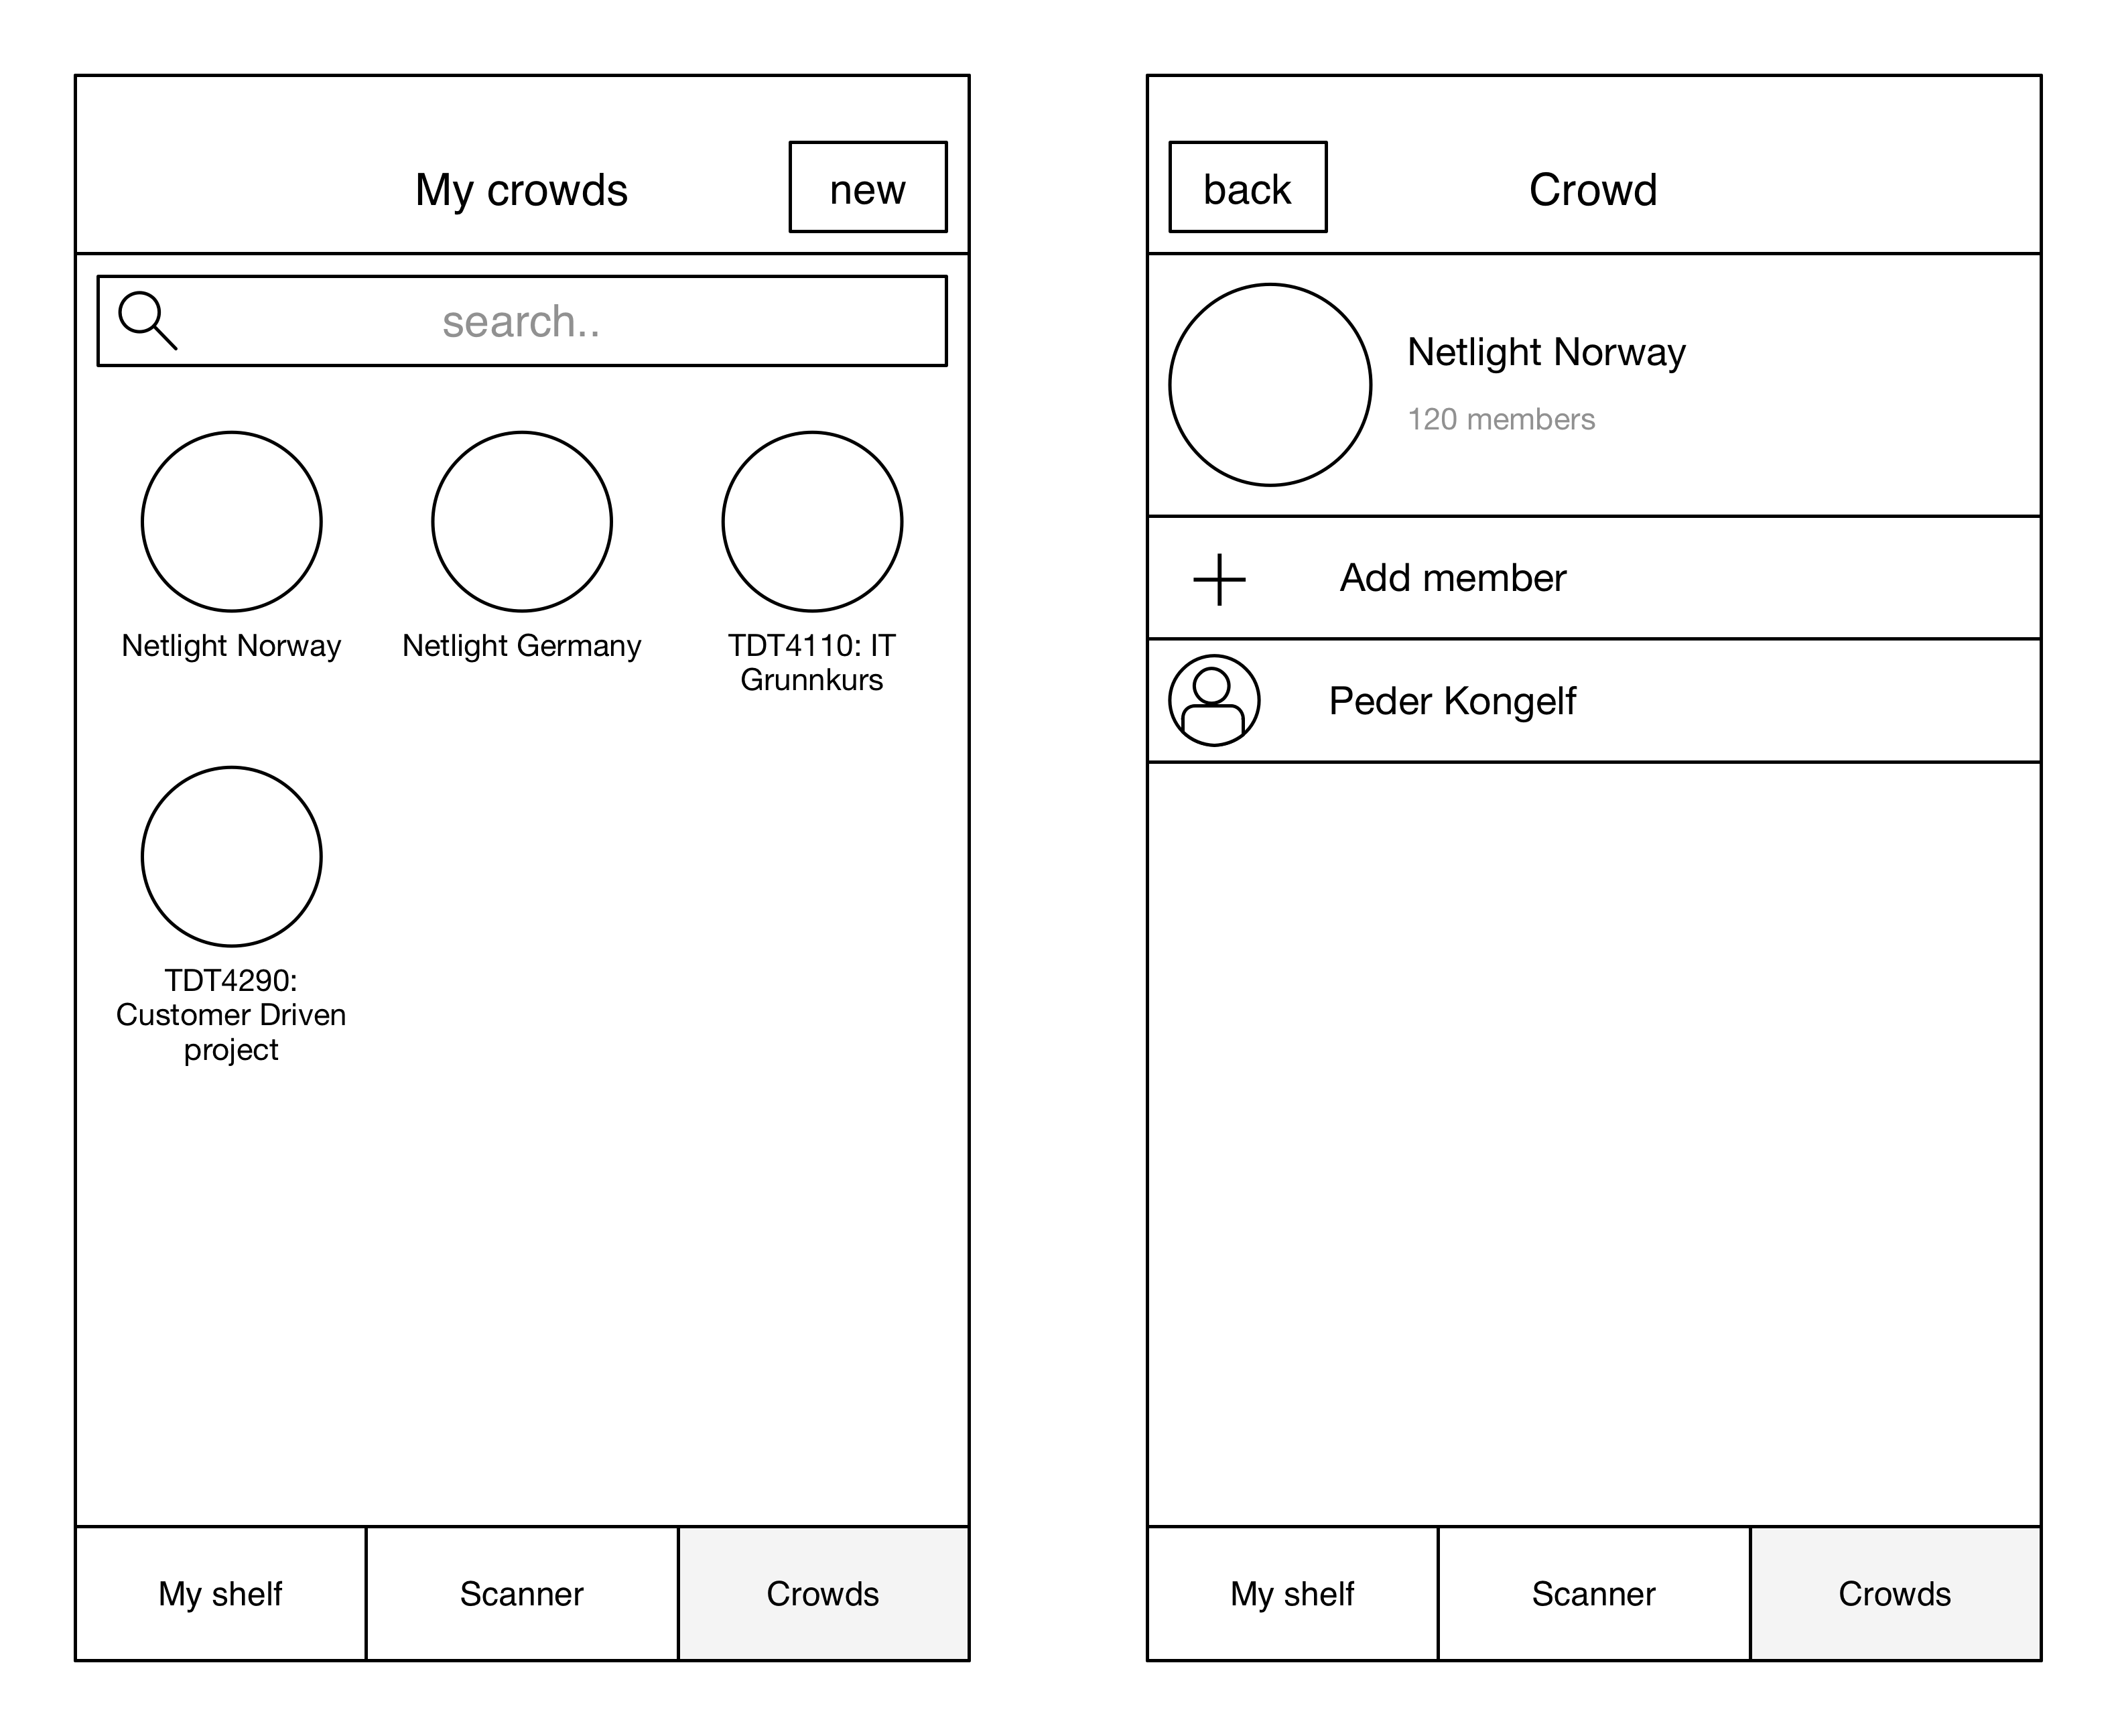
\includegraphics[height=5cm]{figs/v04/Crowd.png}
\caption{The crowd views where the user can see and manage all its crowds}
\label{fig:ios-crowd}
\end{figure}

\begin{figure}
\centering
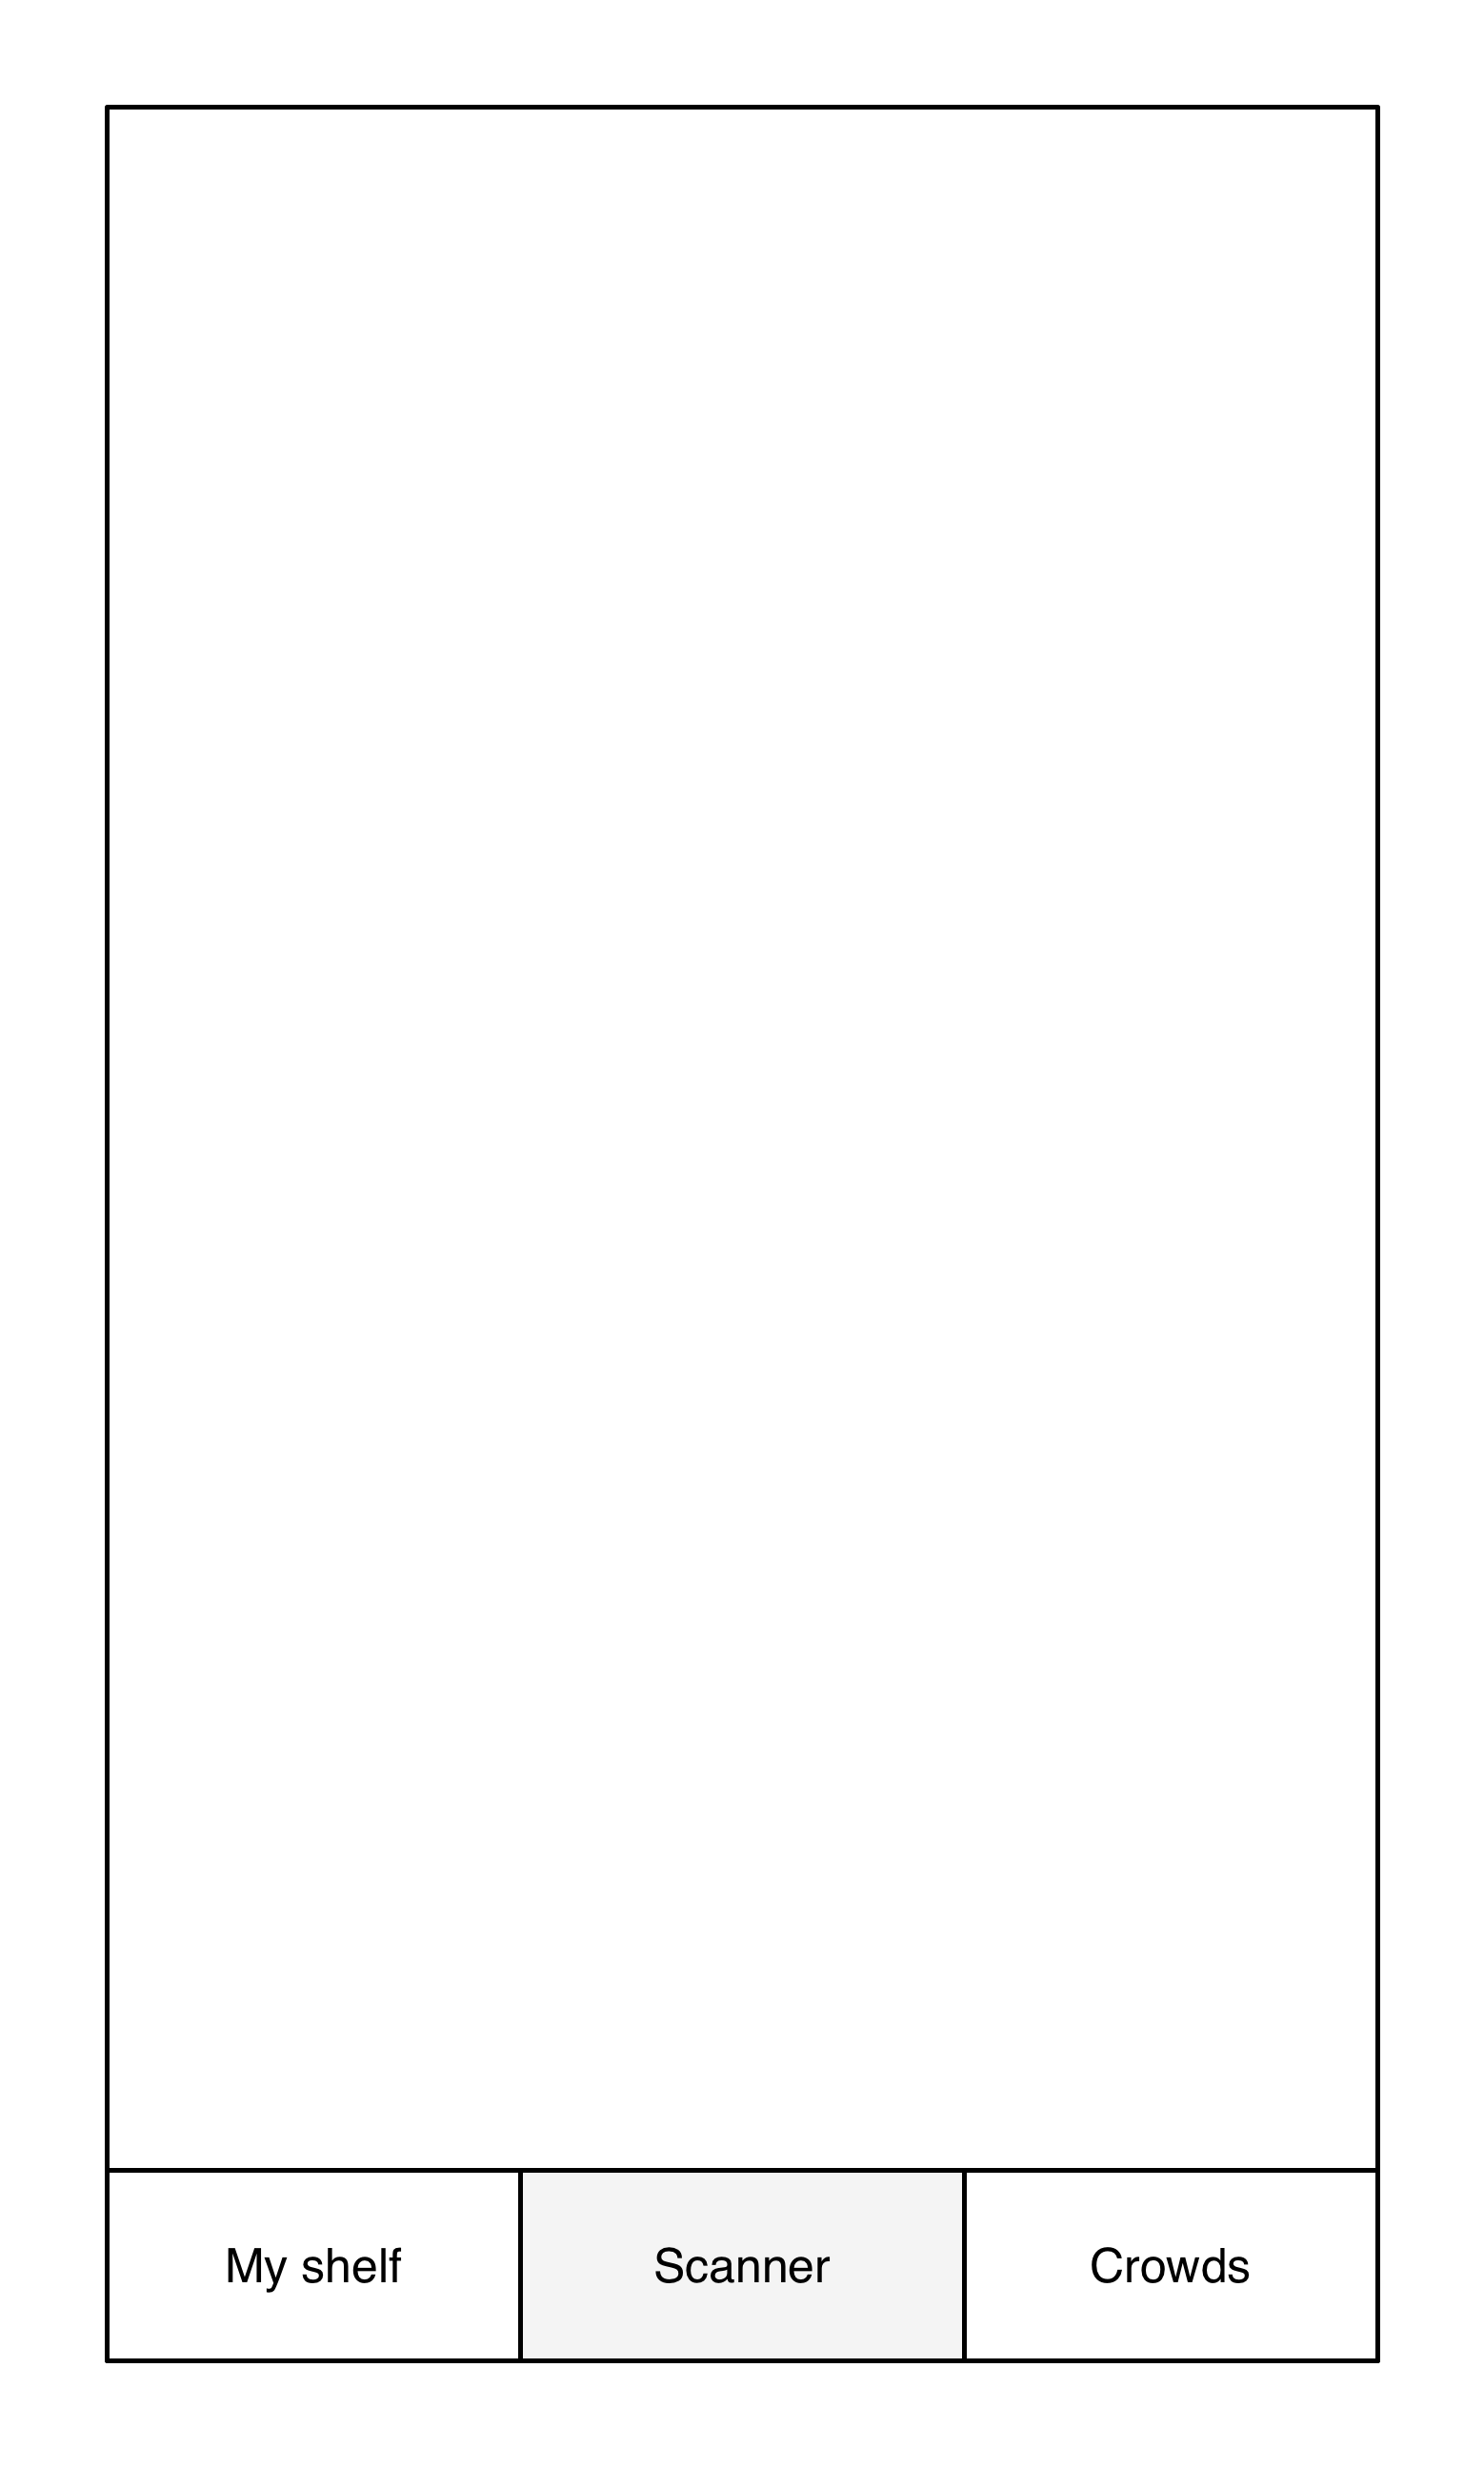
\includegraphics[height=5cm]{figs/v04/Scanner.png}
\caption{The scanner view where the user can scan the books' barcodes}
\label{fig:ios-scanner}
\end{figure}

\begin{figure}
\centering
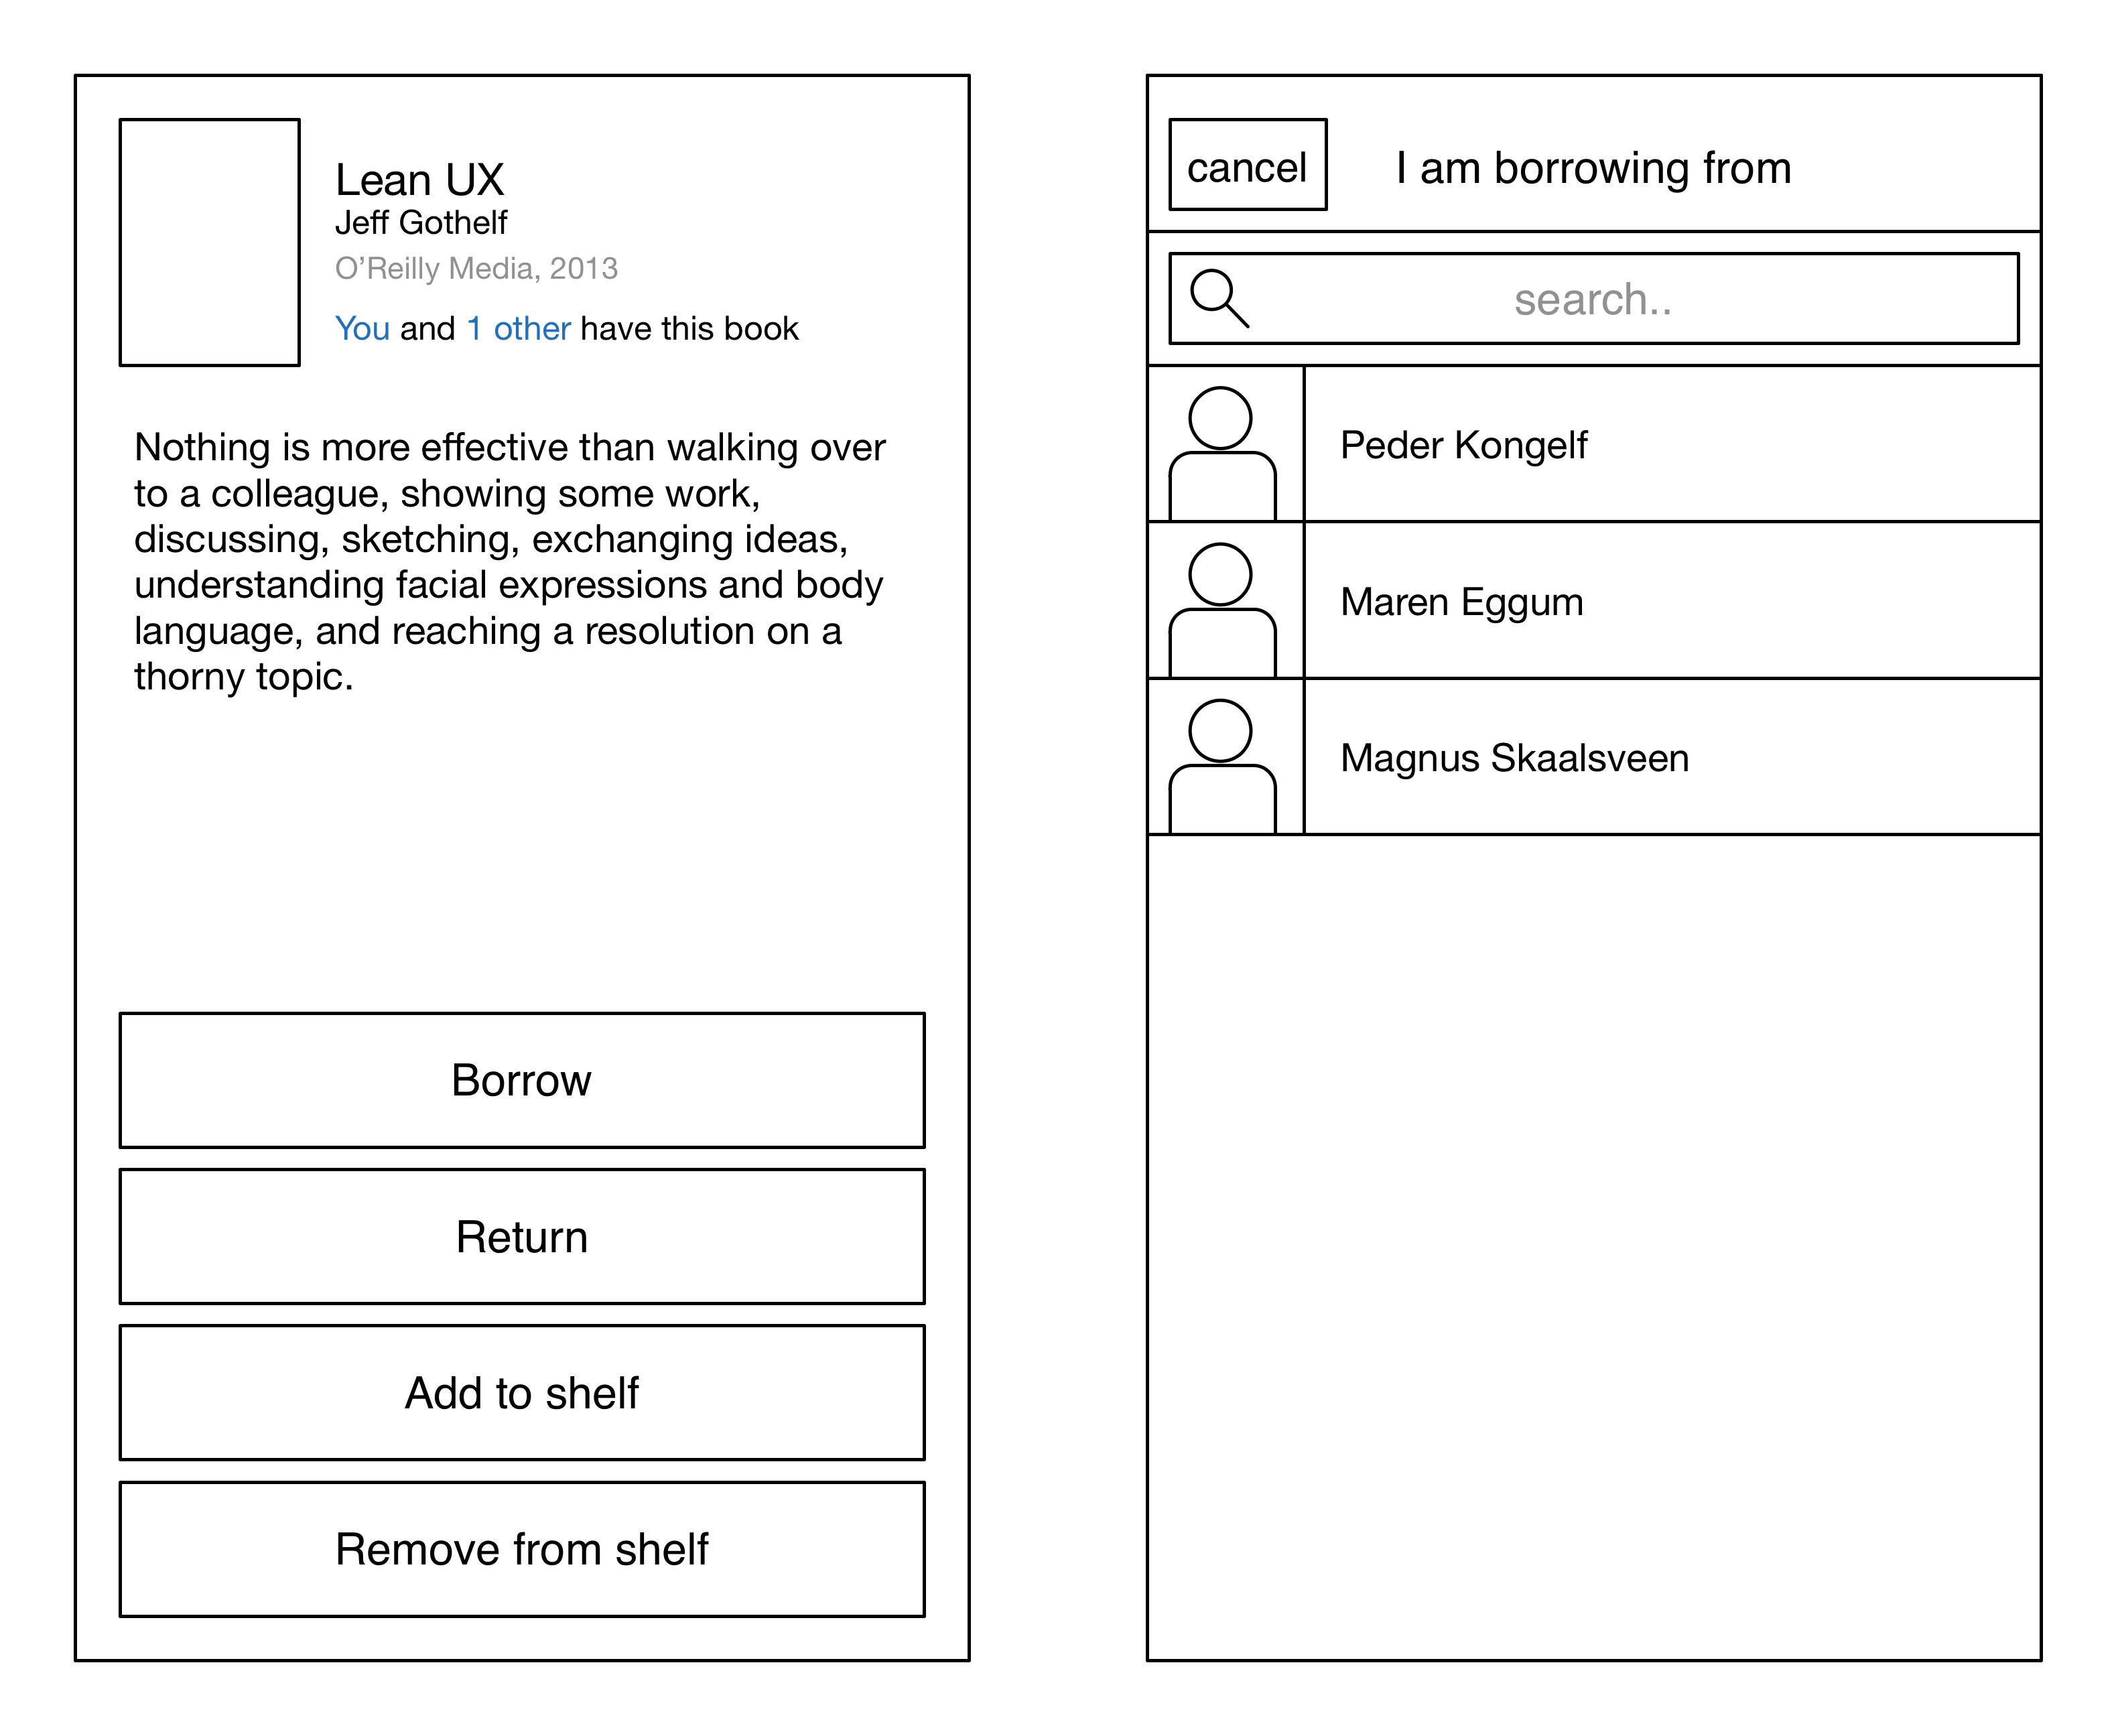
\includegraphics[height=5cm]{figs/v04/Book.png}
\caption{The book view where the user can see information about the book and add or remove it from its shelf.}
\label{fig:ios-book}
\end{figure}

\begin{figure}
\centering
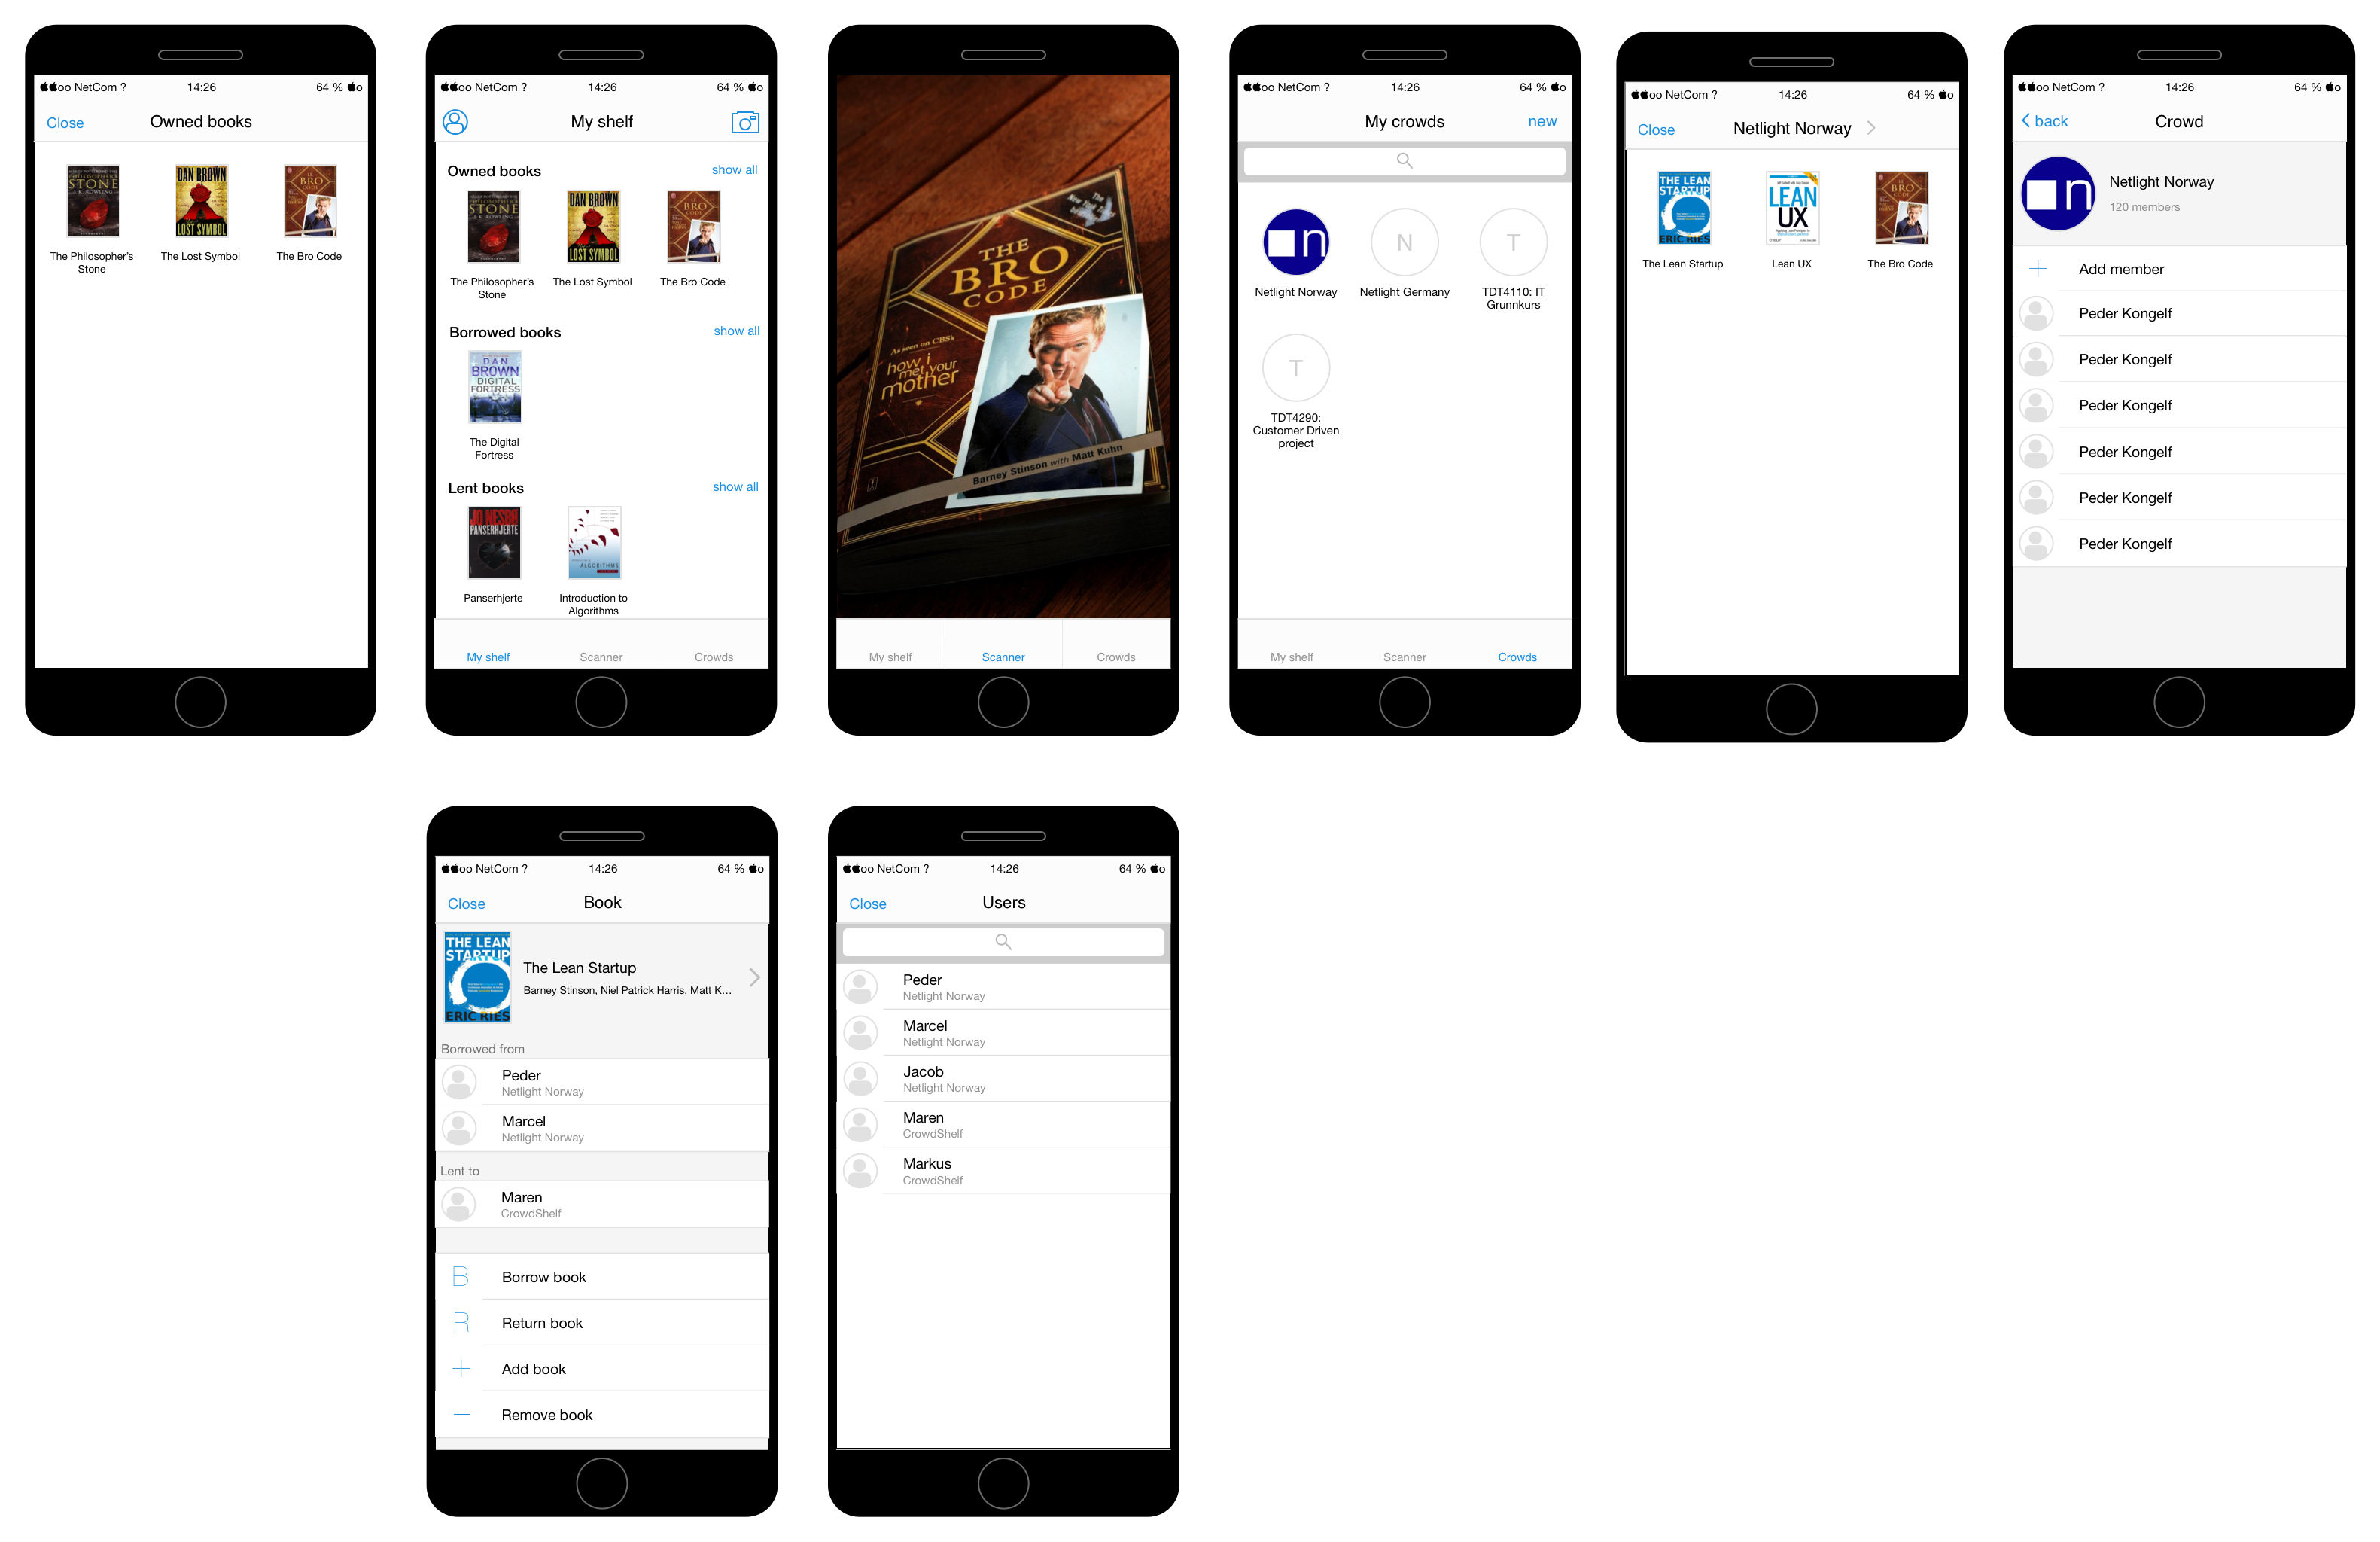
\includegraphics[width=14cm]{figs/v04/detailed-mockup.png}
\caption{A detailed design sketch}
\label{fig:design-sketch-4}
\end{figure}


\subsection{User stories}
\label{user-stories-v4}
This section shows the user stories selected as requirements version 0.4. The stories are selected based on the assumption thought to be the most relevant to test the new features 

\begin{enumerate}
  \item As a user I want to create a crowd
  \item As a user I want to leave a crowd
  \item As a user I want to see all books in my crowds
  \item As a user I want to see the owner and holder of all copies of a book in one/all of my crowds
\end{enumerate}

\subsection{Development}
The team has now gained momentum, and team communication flows better than ever. What this meant for the development of this version, is that the team could work faster. For instance, bugs in the \gls{backend} now fixed on the fly, as the other development teams notified the \gls{backend} lead what was wrong, and the the \gls{backend} team fixed it.

\subsubsection{Android}
\begin{description}
    \item[Features] \hfill\\
The biggest feature of this version was the ability to create new crowds and manage which users that were members of different crowds. A user could be added to a specific crowd by adding a user's username to the crowd, and a user could be a member of multiple crowds. This allowed the user to be able to borrow books from other users in the same crowds. This feature required the application to have a view that could display which crowds a user participates in, and also a view for the creation and management of crowds. 

    \item[Structure] \hfill\\
A new fragment was added to the \code{MainTabbedActivity} activity, which now consisted of three fragments; the user's shelf, the scanner and the new crowd list fragment, \code{CrowdScreenFragment}. See figure \ref{fig:AndroidStructure-04}. The new crowd fragment showed a list of which crowds the user was a member of. It was also possible to click on a crowd to open a new screen where the user could manage crowd details such as name and members. 

\begin{figure}
\centering
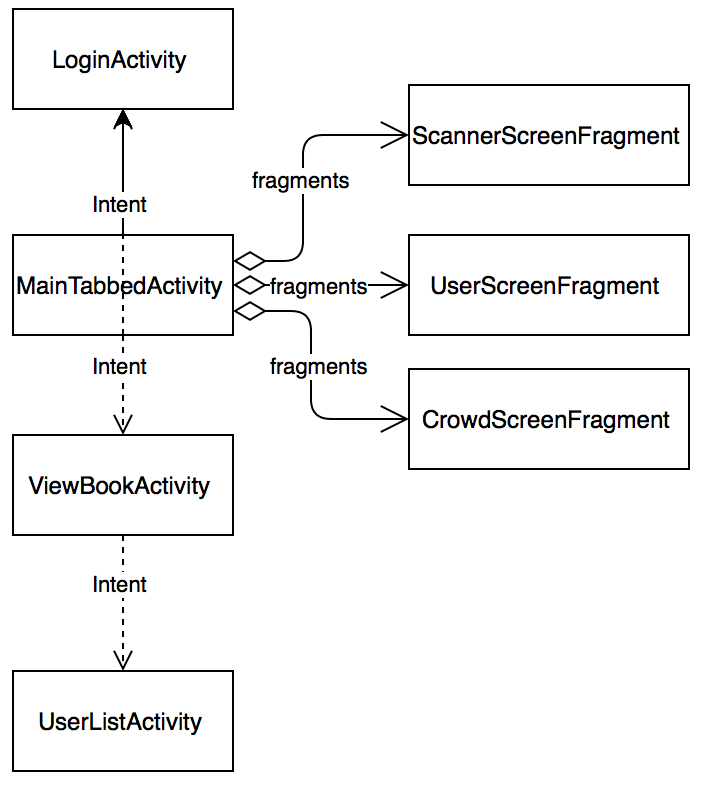
\includegraphics[height=7cm]{figs/v04/AndroidStructure-04.png}
\caption{Basic Android version 0.4 structure}
\label{fig:AndroidStructure-04}
\end{figure}

    \item[Design] \hfill\\
There were not many design changes during this version since the new crowd feature got the teams attention. The team did however start to think about how the application could look, and decided that this was going to be focused on in the next version. One design change that was implemented was to show tabs for the different fragments. Before this version the user was forced to swipe left or right to change fragment, but by implementing tabs, the user could now just go straight to a fragment by tapping on a tab. The new tabs used for navigation can is shown in figure \ref{fig:AndroidDesign-04}

\begin{figure}
\centering
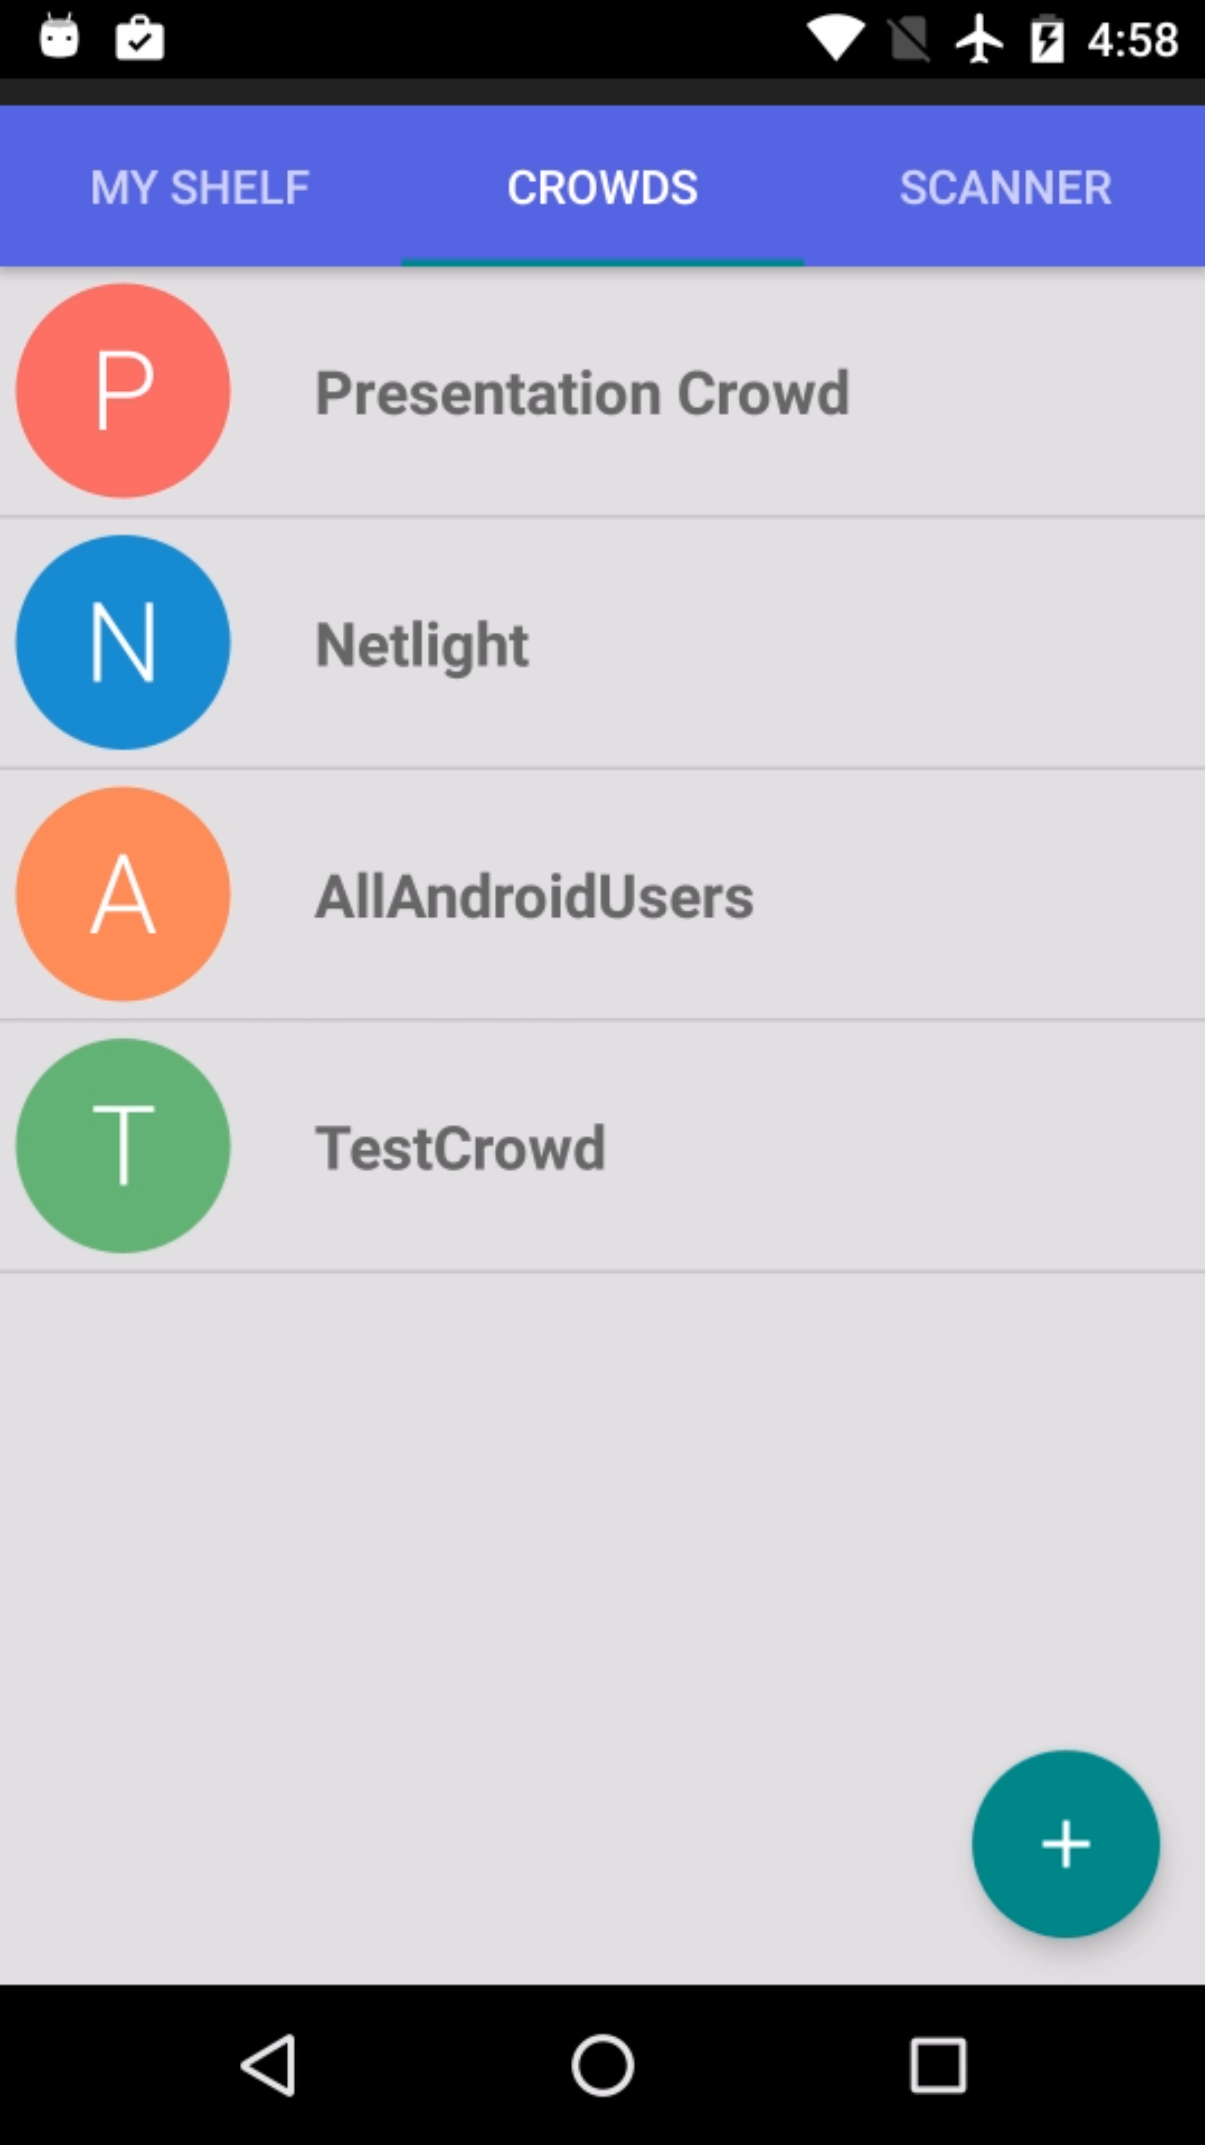
\includegraphics[height=7cm]{figs/v04/AndroidDesign-04.png}
\caption{Android version 0.4 design}
\label{fig:AndroidDesign-04}
\end{figure}

    \item[User feedback] \hfill\\
The new feedback the team wanted to track in this version was if the users used the new implemented crowds functionality.The team then chose to track when a crowd was created, when a a user left a crowd, when a crowd was deleted and when a member was added to a crowd. See table \ref{tab:mixpanel_table} for a full overview of event that got tracked.

    \item[Bug fixes] \hfill\\
The application was made faster on startup by only downloading book information that is not already stored in the local realm database. Another bug discovered was that if a user launched the app, closed it and launched it a second time the application crashed. The reason for this bug was that not all instances using the realm database closed the connection to realm when the instance was finished with communicating with realm. This was solved by making the activities and instances using realm close the connection to realm when the instance was closed or destroyed.
\end{description}

\subsubsection{iOS}
\begin{description}
    \item[Features] \hfill\\
The main feature for this version was to enable users to select which users they wanted to share their books with. This was done by allowing them to create groups and invite other users they trusted. All books a user owned would be shared in all groups they were a part of. In order to achieve this a few new views would have to be created. A new view where the user can see all the groups it is currently a member of, or create new group, and a view with detailed information about the books and members of a given group. 

The network handler had to be updated with methods for creating and removing groups, adding and removing members of a group, and updating information such as the name. 

    \item[Design] \hfill\\
The design of the new views were based on the updated design created after a series of usability tests.

    \item[Feedback] \hfill\\
The integration of Mixpanel from version 0.4 was extended to also include reporting the creation, update and removal of groups. This would allow the team to monitor how the new features were used.
\end{description}

\subsubsection{Backend}
\label{sec:backend-v0.4}
This iteration the team kept up with the other development teams to fix bugs, but most of the time was spent learning about Docker, and creating a Docker-image. \cite{docker} The team managed to write a Docker-file that was used to build a Docker-image. For more information on Docker, see the preliminary studies, section \ref{prelim-docker}. How the Docker-image can be fetched and run is descirbed in the developers documentation to the backend, which is the readme-file of the GitHub-repository. This can be found in appendix \ref{app:backend-readme}.

The team went on to learn about Docker Hub, where you can share Docker-images. \cite{dockerhub} There the team created our own organization page, and a project for the server. \cite{dockerhub-crowdshelf}. The team built the an image for the server application, and pushed it to the Docker Hub. 

Docker Hub lets one can connect with GitHub, so that it detects when someone pushes new code. If the GitHub-repository has a Docker-file, Docker Hub can automatically build a new image and also send HTTP-requests to other services, which in turn can have listeners in place for pulling the image and restarting it's services. \cite{dockerhub-builds} The team set this up so that Docker Hub automatically built a new image whenever there was changes to the \code{master}-\gls{branch} on GitHub.

 In the previous iteration the team bought the domain \url{crowdshelf.xyz} and pointed it to the virtual machine running with Digital Ocean. In this iteration a team member wrote a small application\cite{essoen-dockerpuller} based on one found Online \cite{dockerpuller} that could take in a HTTP-request and based on that call a shell-script. A team member wrote a shell script that could pull the Docker-image from the Docker Hub, and restart it. See code-listing \ref{shell-script} This was set up on the server, and the Docker-image was pulled from the Docker Hub. On the Docker Hub web page the team added a web hook, so that when someone pushed a new version of the Docker-image to the Docker Hub, the Digital Ocean machine automatically pulled the new image, and started it.

In other words the whole deployment process was standardized and automated around the Docker platform with version 0.4.

\begin{lstlisting}[float,floatplacement=H,frame=single, columns=fullflexible, caption=Shell-script used by the virtual machine running at Digital Ocean to restart the server application with Docker when there is deployed a new version, label=shell-script]
    docker pull crowdshelf/server:latest
    docker stop crowdshelf
    docker rm crowdshelf
    docker run --name crowdshelf --net host crowdshelf/server:latest
\end{lstlisting}


This version was also spent discussing a possible new service that was to be developed: A Book Service. A web developer from our customer wanted to build a web application on top of the CrowdShelf \gls{API}. The problem here was that the web application did not have local storage, and therefore had difficulties cashing the data from the Google Books \gls{API}, that the mobile applications used for meta information. The web developer also claimed that the Google Books \gls{API} had some limitations as to how many requests one could run. The customer requested that the team developed a new service that could save Google Books-data, and connect it with the already existing \gls{backend}. The team also found that the \gls{backend} could be a service to save books that were not anywhere else. The customer representative also suggested that other types of items could be saved in the service, which in turn could be used to extend the market of the application. 

The team developed a specification for an \gls{API} together with the customer representative that could meet the above mentioned needs. The team soon found it to be very complex. If one would have Google Books references in an own database, and a reference to them from the already existing \gls{backend}, a lot of validation had to be implemented. The backend team also had some difficulties seeing the need of the web developer. The problem she had, did not indicate that she would need a new service. The mobile application developers did multiple requests to the Google Books API, and met no limitations, while the web developer claimed she did. The team found that this may have to do with a limitation the Google Books \gls{API} had with searching their databases. The team could request resources directly as much as as the team wanted.

After a final meeting with the customer representative, the \gls{backend} team an the customer finally decided to scrap the plans for the service, as it would be too complex and costly to develop in the time frame of the project. 

\subsection{Feedback}
Feedback from the survey (appendix \ref{app:0.4-survey-feedback}) was a clear indication that users want some way of restricting the access other users have to their virtual library. Only 6 \% were willing to share their books with strangers, but 80 \% wanted to share books with friends and colleagues. This seemed to support the theory that allowing users to create groups, in which they could share their books, was a demand rooted in future user needs.


The results from the usability tests were highly dependent on the user group in question. All students had no problem navigating the application, and completion all tasks. This could be a consequence of the design being based on Facebook's Messenger application design, which  students probably use more than most other user groups. The employees at \gls{IDI} had some trouble understanding the applications in the beginning of the test. In particular, they had a hard time understanding that they could interact with the tab bar. As soon as they realized this, all but one completed the rest of the tasks without hesitation. 


The last tester did not manage to complete any task, and spent a long time just looking at the views. There could be many reasons for this. Perhaps she was having trouble understanding the concept of a paper prototype test, did not understand the basic concept and purpose of the application, or simply did not understand how to use the application the team presented. As no other users have expressed that they do not understand the most basic concepts of the solution, the team assumed that the latter was the most likely. Therefore a new design was created where some of the buttons were made more prominent. 


Like in previous versions, the applications were uploaded to Google Play and TestFlight, but very few users ever downloaded or installed them. During the customer meeting, the customer representative seemed satisfied with the result of the version, so the team continued the effort in developing a minimal viable product. Before this is achieved, there will be no usage data to measure.

Minutes from the customer meetings are located in \ref{app:customer-minutes-8} and \ref{app:customer-minutes-9}.


\begin{figure}
\centering
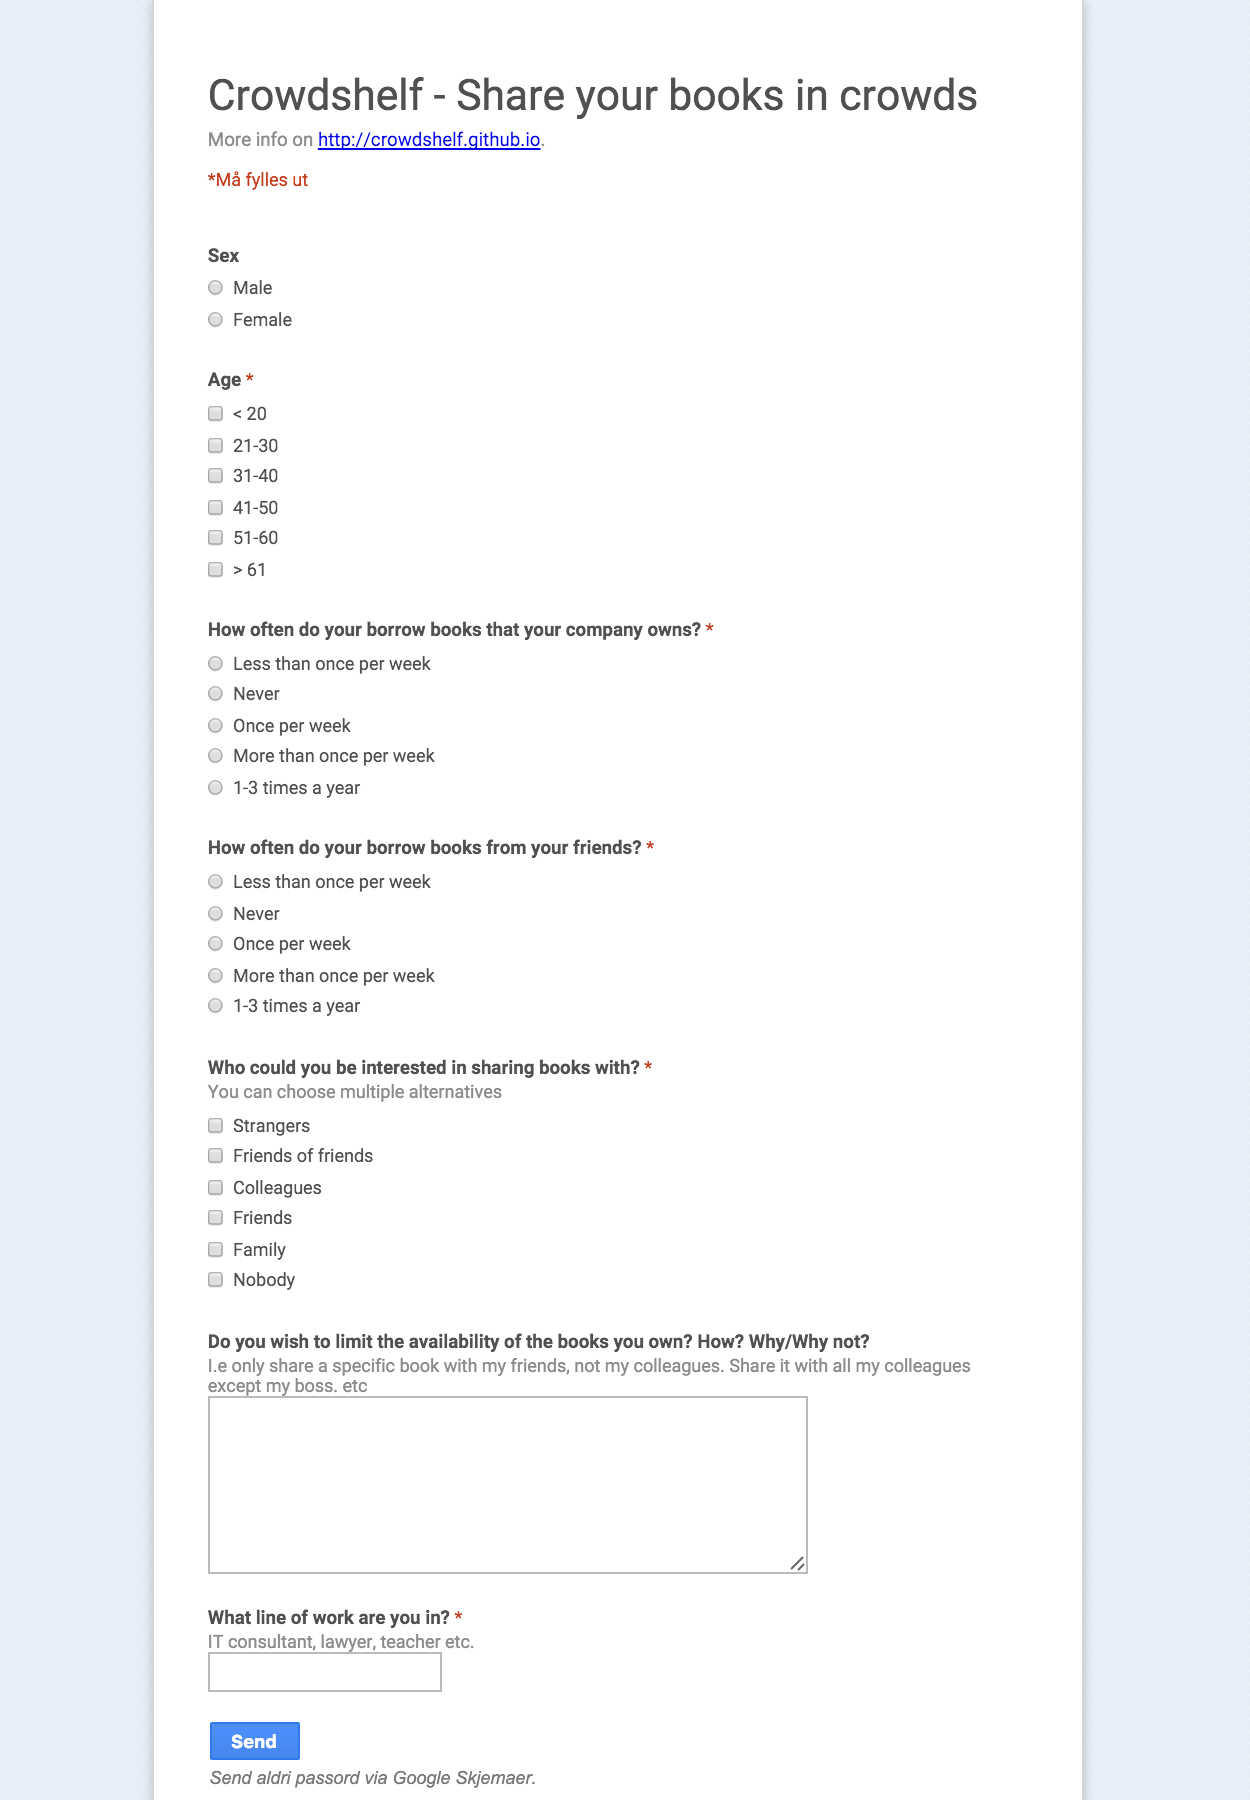
\includegraphics[height=\textheight]{figs/v04/survey.png}
\caption{The survey used to gather necessary information from potential users}
\label{fig:0.4-survey}
\end{figure}

\begin{figure}
\centering
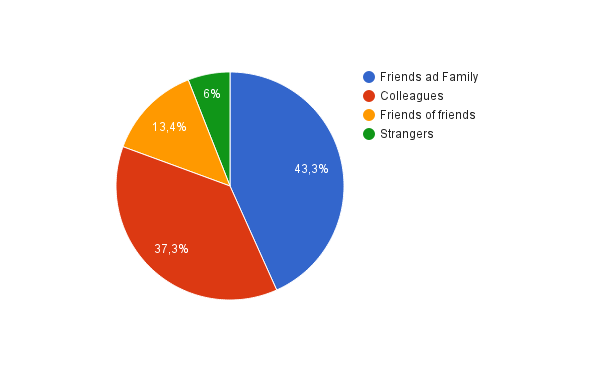
\includegraphics[width=\textwidth]{figs/v04/feedback-pie.png}
\caption{A pie chart illustrating the percentages of people willing to share with certain groups}
\label{fig:0.4-survey-feedback}
\end{figure}


\subsection{Version progress}

With the completion of this version, the application is one step closer to being ready for distribution. The crowd feature enables users to choose how they want to share their books. The progression during this iteration is illustrated in figure \ref{fig:0.4-survey-feedback}. A complete list of all tasks from this version can be seen in the release note in appendix \ref{app:release-note-4}

Although no serious problems were encountered, this iteration lasted more than a week due to the delivery of a mid-term report. A few days were spent solely on preparing the report which lead to a halt in the development on both the clients and the backend. 

A new blog post was written and is displayed in figure \ref{fig:blog-week-eight}

\begin{figure}
\centering
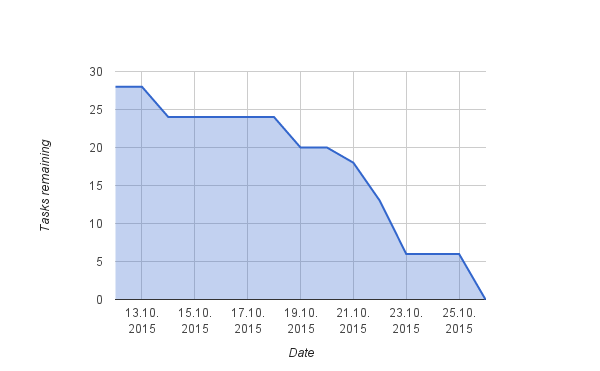
\includegraphics[width=\textwidth]{figs/v04/version-progress-4.png}
\caption{Task progress version 0.4}
\label{fig:version-progress-4}
\end{figure}

\begin{figure}
\centering
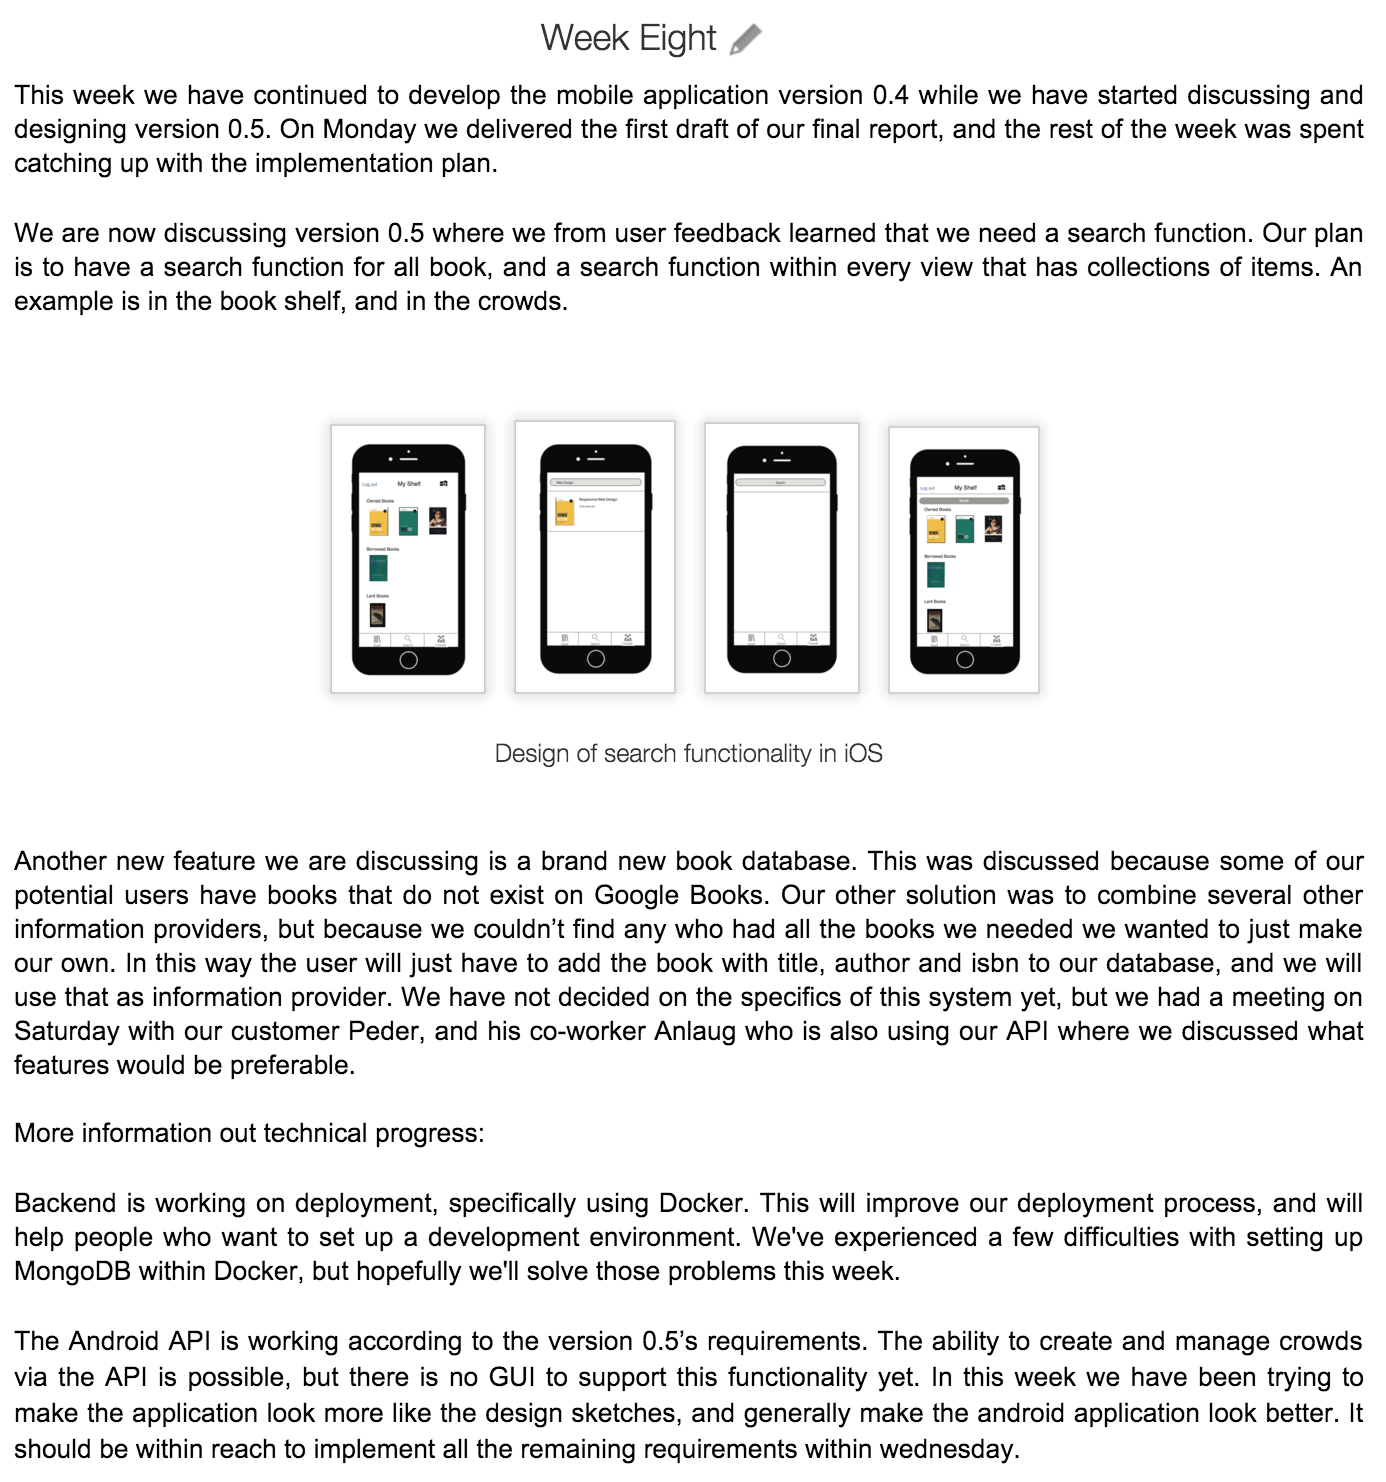
\includegraphics[height=20cm]{figs/v04/WeekEight.png}
\caption{Blog post from week eight}
\label{fig:blog-week-eight}
\end{figure}

\subsection{Review and retrospective}

At the end of the iteration, the mobile applications and \gls{API} were presented to the customer. For Android and iOS, a couple of videos demonstrating the crowds feature were made. The customer representative seemed pleased with the solution, but he suggested that the team should attempt to establish a vocabulary to ease the communication when discussing subjects such as groups, end points, and crowds. He also wanted the demonstration videos to contain books which a broader audience would recognize, and use crowd names that could help the viewer understand how the crowd feature can be used. The minutes from the customer meetings is located as appendix \ref{app:customer-minutes-8} and \ref{app:customer-minutes-9}.

Because the final delivery was merely two weeks away, the customer representative shared what his functional requirements for the end result were. I addition to the existing features, it needs to be possible to search for books using raw text. This could be done using the Google Books API, but it should be possible to filter the results to contain only books from the users crowds. The last requirement was that users had to be authenticated in order to restrict what data a people have access to. At the moment, everyone has access to all information in the database provided they have the necessary usernames and \gls{ISBN}s. These features should be implemented during the last two iterations.

The focus points of this iteration were to become better at using Jira for tracking issues, and connecting our results to the initial assumption. All team members agreed that during the this version, they had become better at using Jira, and could now see the connection between the assumptions and results.

\begin{figure}
\centering
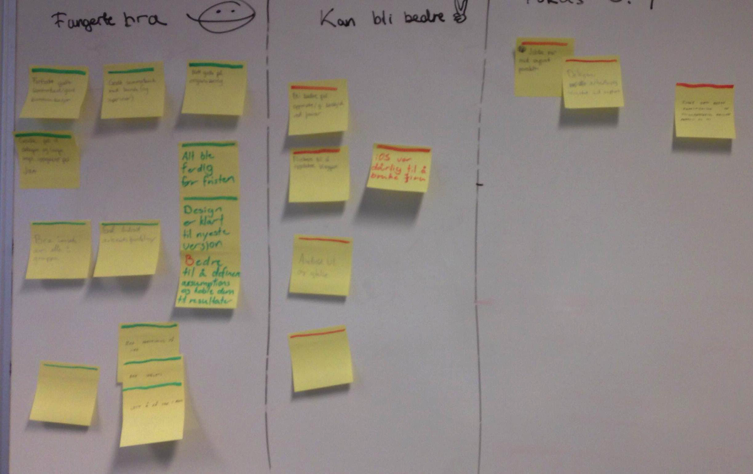
\includegraphics[height=8cm]{figs/v04/retrospective.png}
\caption{The board after the retrospective meeting in version 0.4}
\label{fig:retrospective-4}
\end{figure}


\subsection{Summary}
The initial assumption for this version was that users only want to share books with a selection of users. Even though users said that they do not want any restrictions on their books, the survey was a clear indication that they do not want to share with strangers. This told the team one of the lessons learned this version: users want to restrict who can borrow their books.

The crowd functionality was implemented on the clients and on the server based on this knowledge, and then distributed to users through Google Play and TestFlight.\cite{google-play}\cite{testflight} When usage data is received, question eight can be answered as well.
